En esta práctica se aborda el filtro de partículas. Se trata de un algoritmo eficiente para calcular la localización de un robot móvil que dispone de sensores de distancia.

\section{Código Implementado}
El algoritmo se basa en la generación de una serie de partículas empleando como centro la posición ideal (posición estimada) y siguiendo una distribución de probabilidad
sobre un radio indicado como parámetro. Sobre esta distribución inicial, iterativamente se aplica el movimiento del robot y se actualiza la probabilidad de cada partícula, 
tras lo que se realiza un remuestreo, en el que se escogen las partículas con mayor probabilidad.


\subsection{Análisis}
El código proporcionado contiene muchas de las funciones necesarias. Para el correcto funcionamiento se implementan las siguientes funciones:
\begin{itemize}
  \item \texttt{genera\_filtro}: Se inicializa el filtro de partículas con el tamaño indicado, para ello se crea un array de robots, siendo
cada uno una partícula. Se inicializa cada partícula con un ruido arbitrario, y se asigna una posición siguiendo una distribución uniforme en el área
descrita por el centro y el radio indicados. Adicionalmente, la orientación se establece añadiendo un ruido gausiano a la orientaión ideal. Por último,
se establece la probabilidad de cada partícula en base a las mediciones y las balizas.
  \item \texttt{dispersion}: Considera la dispersión espacial de las partículas, para ello, se retorna un array conteniendo los valores mínimos y máximos de las componentes x e y de las posiciones de todas las partículas.
  \item \texttt{peso\_medio}: Se calcula el peso medio empleando la suma de todos los pesos para normalizar el de cada partícula.
\end{itemize}
Todas estas funciones se observan en las figuras \ref{fig:genera_filtro}, \ref{fig:dispersion} y \ref{fig:peso_medio}.

\begin{figure}[htb]
  \centering
  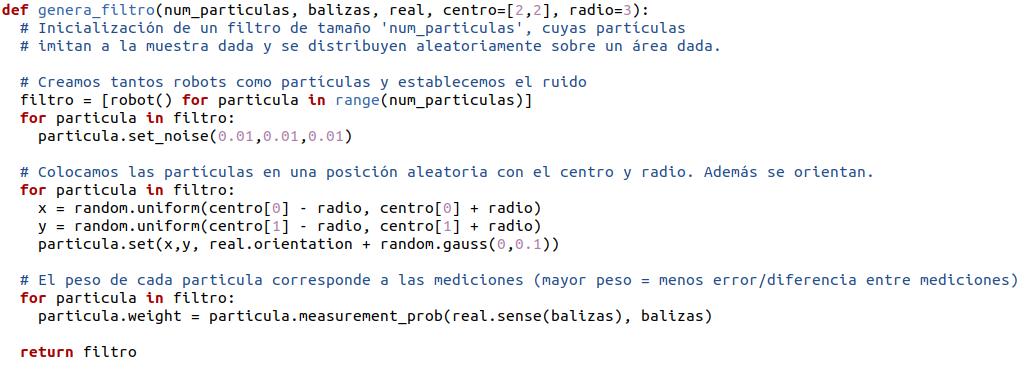
\includegraphics[width=1\linewidth]{images/filtroc1.png}
  \caption{Función \textit{genera\_filtro}}
  \label{fig:genera_filtro}
\end{figure}
\begin{figure}[htb]
  \centering
  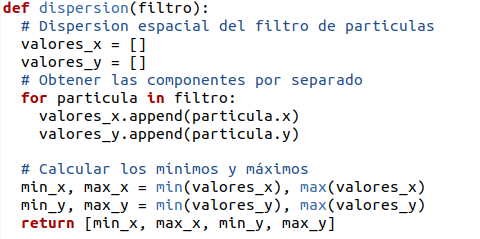
\includegraphics[width=.5\linewidth]{images/filtroc2.png}
  \caption{Función \textit{dispersion}}
  \label{fig:dispersion}
\end{figure}
\begin{figure}[htb]
  \centering
  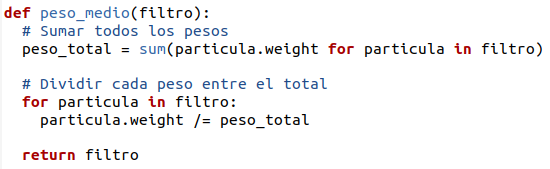
\includegraphics[width=.6\linewidth]{images/filtroc3.png}
  \caption{Función \textit{peso\_medio}}
  \label{fig:peso_medio}
\end{figure}

Además, en el programa principal se codifican los siguientes comportamientos:
\begin{itemize}
  \item \texttt{inicialización del filtro}: se crea el filtro empleando la función \textit{genera\_filtro}, usando el número de partículas inicial indicado como parámetro. Se toma además como centro la posición inical del robot, y se emplea un radio 1.
A continuación se establece como posición inicial la partícula más probable, y se inicializan la trayectoria ideal y real. El código de esta sección se muestra en la figura \ref{fig:inicializacion}.
  \item \texttt{actualización de la trayectoria y las probabilidades}: se mueven todas las partículas del filtro con el vector de movimiento calculado para dirigirse hacia el objetivo. A continuación,
se actualizan los pesos con las nuevas probabilidades, y se normalizan empleando la función \textit{peso\_medio}. Finalmente se actualiza la trayectoria real e ideal. El código de este fragmento así como 
del remuestreo se encuentra en la figura \ref{fig:actualizacion}.
  \item \texttt{remuestreo}: se emplea la función ya definida "resample", que toma como parámetros el filtro y el número de partículas deseado. 
\end{itemize}
\begin{figure}[htb]
  \centering
  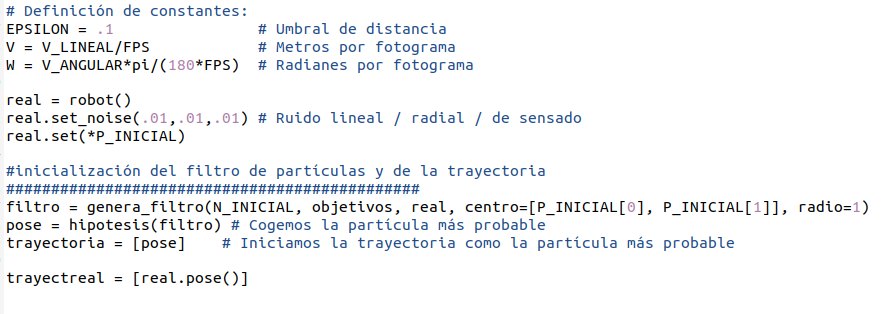
\includegraphics[width=1\linewidth]{images/filtroc4.png}
  \caption{Inicialización del filtro} 
  \label{fig:inicializacion}
\end{figure}
\begin{figure}[htb]
  \centering
  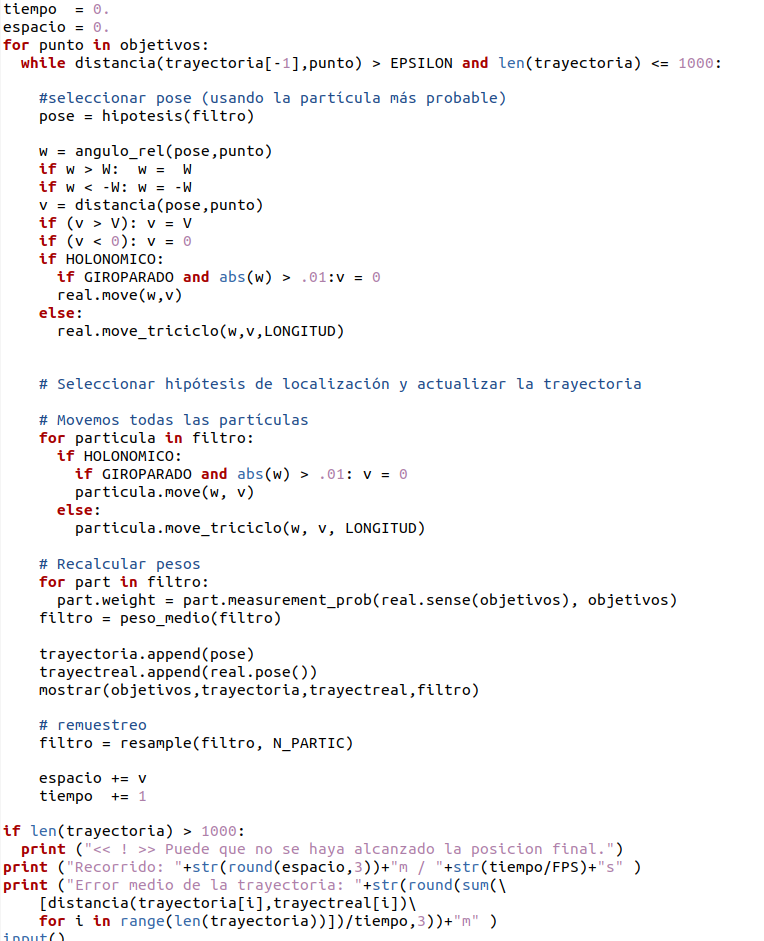
\includegraphics[width=.9\linewidth]{images/filtroc5.png}
  \caption{Actualización del filtro y remuestreo}
  \label{fig:actualizacion}
\end{figure}

\subsection{Complejidad}
El costo computacional del algoritmo depende principalmente del número de partículas que se mantienen en el filtro, el cuál es uno de los principales
parámetros a ajustar. En general, el algoritmo es lineal en el número de partículas, ya que en cada iteración se actualiza la posición y probabilidad de cada partícula.
%%%%%%%%%%%%%%%%%%%%%%%%%%%%%%%%%%%%%%%%%%%%%%%%%%%%%%%%%%%%%

\section{Mejoras}
No se han implementado mejoras, pero se proponen las siguientes:
\begin{itemize}
  \item \texttt{Número variable de partículas}: Emplear un enfoque adaptativo, en el que el número de partículas se ajuste en función
de la precisión del modelo (la probabilidad de que la posición predicha sea correcta según las mediciones).
  \item \texttt{Lectura de datos de configuración desde un JSON}: al igual que en prácticas anteriores, se podría emplear un fichero de configuración para evitar tener
que modificar el código cuando se quieren alterar parámetros como el número de partículas, el radio de dispersión, etc.
  \item \texttt{Mejoras del remuestreo}: ahora mismo se implementa un remuestreo básico, sería interesante considerar aproximaciones más inteligentes, como 
por ejemplo, remuestreo estratificado, en el que se busca mejorar la representatividad de las partículas escogidas.
\end{itemize}

%%%%%%%%%%%%%%%%%%%%%%%%%%%%%%%%%%%%%%%%%%%%%%%%%%%%%%%%%%%%%
\section{Ejemplos de ejecución}
Se han realizado varios experimentos sobre la trayectoria con 3 balizas.
\subsection{Ejemplo 1}

Realizamos una ejecución para comprobar el funcionamiento con los valores por defecto, destacando que el tamaño inicial del filtro es de 2000 partículas, y el tamaño el resto de las iteraciones es de 50.

Observamos en la figura \ref{fig:ejemplo1} el inicio del experimento, en el que se observa la posición inicial del robot y las partículas generadas. En la figura \ref{fig:ejemplo2} se muestra la segunda iteración, en la que se observa la reducción del número de partículas.
En la figura \ref{fig:ejemplo3} se muestra el progreso del experimento, destacando la existencia de tres grupos de partículas, unas por encima de la posición real, otras simétricamente por debajo, y el resto en la posición real. Esto se debe a la ambigüedad de las mediciones con la configuración de las balizas.
En la figura \ref{fig:ejemplo4} se muestra la convergencia del experimento, en la que se observa que las partículas se concentran en la posición real del robot. Por último, en la figura \ref{fig:ejemplo5} se muestra la trayectoria del robot, en la que se observa que el filtro de partículas ha sido capaz de seguir la trayectoria real del robot.

%%%%%%%%%%%%%%%%%%%%%%%%%%%
\begin{figure}[htb]
  \centering
  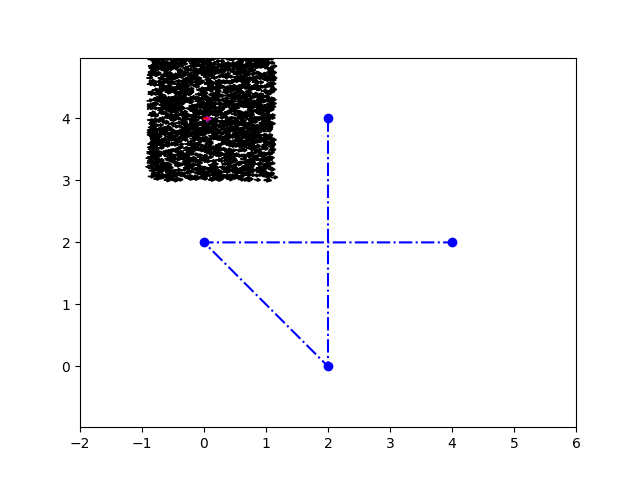
\includegraphics[width=.8\linewidth]{images/filtro1.png}
  \caption{Inicio del ejemplo 1}
  \label{fig:ejemplo1}
\end{figure}
\begin{figure}[htb]
  \centering
  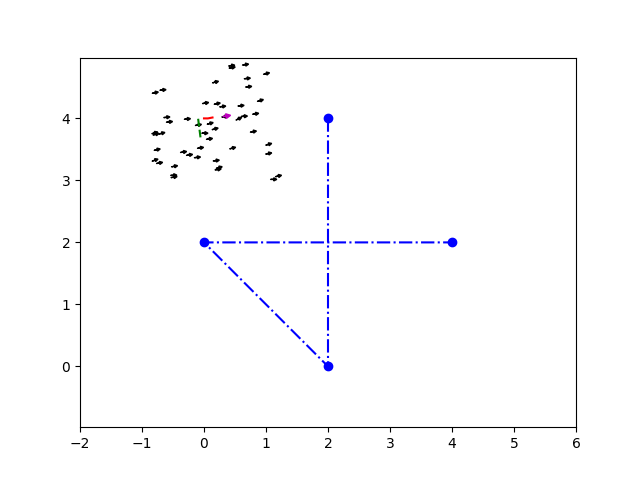
\includegraphics[width=.8\linewidth]{images/filtro2.png}
  \caption{Segunda iteración del ejemplo 1}
  \label{fig:ejemplo2}
\end{figure}
\begin{figure}[htb]
  \centering
  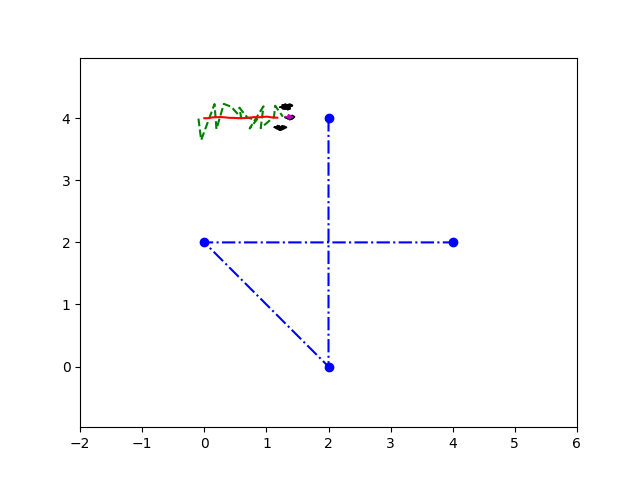
\includegraphics[width=.8\linewidth]{images/filtro3.png}
  \caption{Progreso del ejemplo 1}
  \label{fig:ejemplo3}
\end{figure}
\begin{figure}[htb]
  \centering
  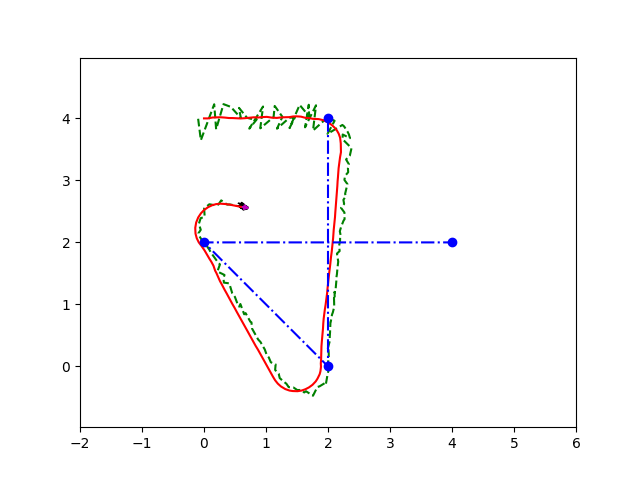
\includegraphics[width=.8\linewidth]{images/filtro4.png}
  \caption{Convergencia del ejemplo 1}
  \label{fig:ejemplo4}
\end{figure}
\begin{figure}[htb]
  \centering
  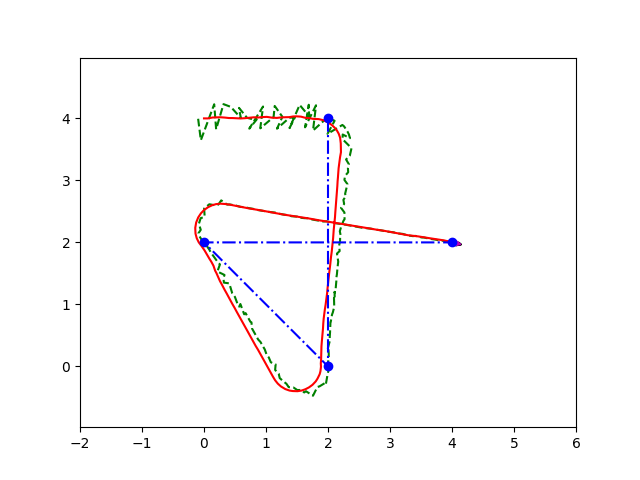
\includegraphics[width=.8\linewidth]{images/filtro5.png}
  \caption{Trayectoria del ejemplo 1}
  \label{fig:ejemplo5}
\end{figure}
%%%%%%%%%%%%%%%%%%%%%%%%%%%
\subsection{Ejemplo 2}
Se repite el experimento anterior, manteniendo el número de partículas inicial, pero con un tamaño de 100 del filtro de partículas en ejecución. En la figura \ref{fig:ejemplo7} se observa que en las primeras iteraciones ya no existe la 
ambigüedad del ejemplo previo, sino que se ve un grupo cercano de partículas. En la figura \ref{fig:ejemplo8} se observa la convergencia del experimento, que ha tenido lugar más rápido que en el anterior ejemplo. Por último, en la figura \ref{fig:ejemplo9} se muestra la trayectoria del robot, en la que se observa que el filtro de partículas ha sido capaz de seguir la trayectoria real del robot con mayor precisión, no obstante, 
cabe destacar que el coste computacional ha sido mayor, el experimento ha tardado más tiempo.
\begin{figure}[htb]
  \centering
  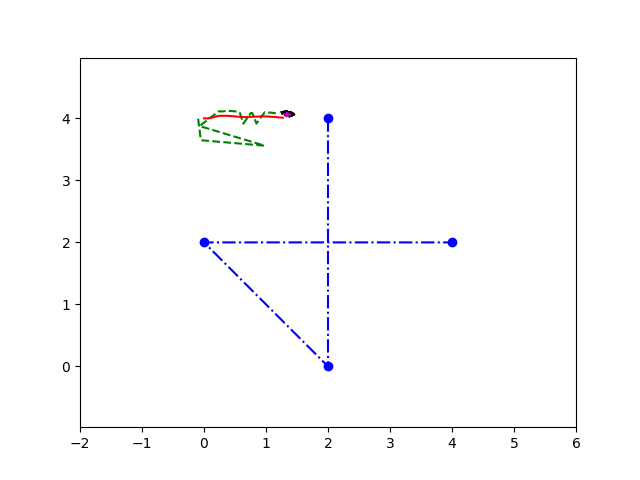
\includegraphics[width=.8\linewidth]{images/filtro7.png}
  \caption{Inicio del ejemplo 2}
  \label{fig:ejemplo7}
\end{figure}
\begin{figure}[htb]
  \centering
  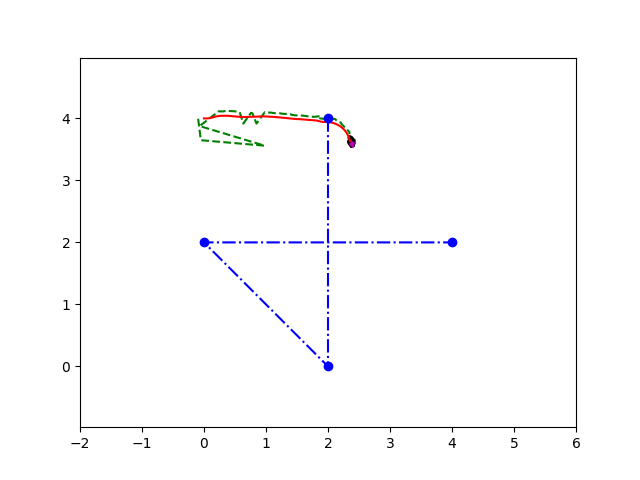
\includegraphics[width=.8\linewidth]{images/filtro8.png}
  \caption{Convergencia del ejemplo 2}
  \label{fig:ejemplo8}
\end{figure}
\begin{figure}[htb]
  \centering
  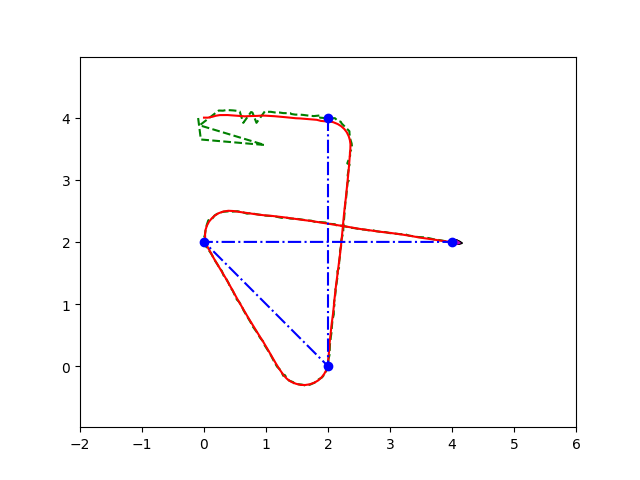
\includegraphics[width=.8\linewidth]{images/filtro9.png}
  \caption{Trayectoria del ejemplo 2}
  \label{fig:ejemplo9}
\end{figure}
%%%%%%%%%%%%%%%%%%%%%%%%%%%
\subsection{Ejemplo 3}
A continuación se repite el experimento pero para un filtro con tamaño 10.
En la figura \ref{fig:ejemplo10} se observa la trayectoria del experimento. Destaca que la precisión es mucho menor a los experimentos anteriores, y mientras que se converge rápidamente, 
se pierde la trayectoria real del robot en varias ocasiones.
\begin{figure}[htb]
  \centering
  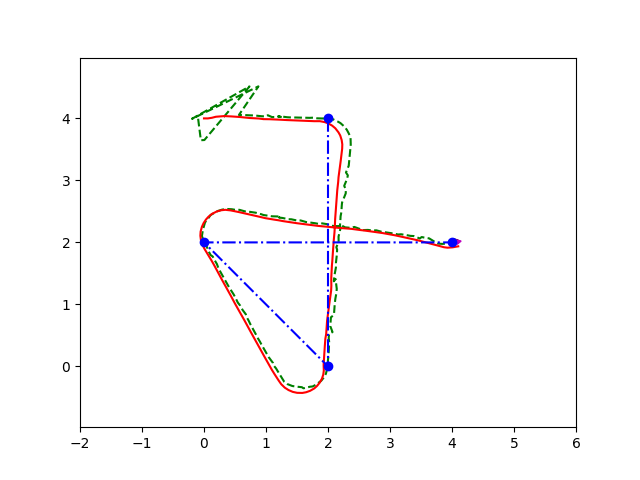
\includegraphics[width=.8\linewidth]{images/filtro10.png}
  \caption{Trayectoria del ejemplo 3}
  \label{fig:ejemplo10}
\end{figure}
%%%%%%%%%%%%%%%%%%%%%%%%%%%%%%%%%%%%%%%%%%%%%%%%%%%%%%%%%%%%%
\section{Conclusions}
We have implemented a simple particle filter and proved its functionality with some examples. We have studied the computational complexity of the algorithm and seen that
a higher particle count leads to a higher precision, but also to a higher computational cost. It seems that 50 particles is a good balance between precision and performance.
It is also worth noting that this algorithm is a fast approach for localization of a moving robot, being faster than the approach described in chapter 4.
%%%%%%%%%%%%%%%%%%%%%%%%%%%%%%%%%%%%%%%%%%%%%%%%%%%%%%%%%%%%%

